% Hevea - ITILv3 Resumo
% An ITILv3 overview.
%
% Author: José Lopes de Oliveira Jr. <jilo.cc>
%
% LICENSE
% This program is free software: you can redistribute it and/or modify
% it under the terms of the GNU General Public License as published by
% the Free Software Foundation, either version 3 of the License, or
% (at your option) any later version.
%
% This program is distributed in the hope that it will be useful,
% but WITHOUT ANY WARRANTY; without even the implied warranty of
% MERCHANTABILITY or FITNESS FOR A PARTICULAR PURPOSE.  See the
% GNU General Public License for more details.
%
% You should have received a copy of the GNU General Public License
% along with this program.  If not, see <http://www.gnu.org/licenses/>.
%%


\chapter{Melhoria de Serviço Continuada}
\label{cha:melhoria}


\begin{figure}
    \centering
    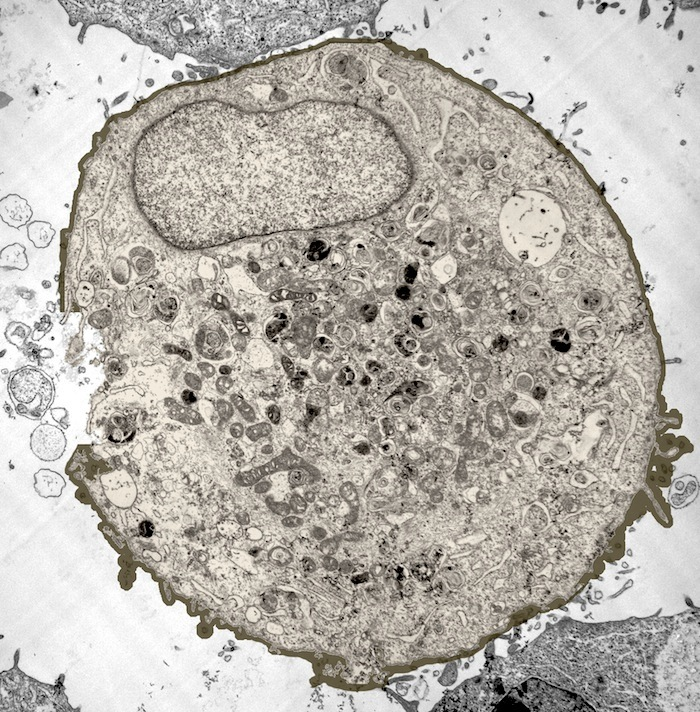
\includegraphics[width=0.7\textwidth]{img/prostate_cancer}\\
    {\scriptsize Prostate Cancer --- Georgia Tech}
\end{figure}

Tem por objetivo proporcionar um guia prático para aumentar a eficiência,
maximizar a efetividade e otimizar o custo dos processos subjacentes ao
Gerenciamento de Serviço de TI e seus processos subjacentes em 3 níveis dentro
da organização: o bom funcionamento do Gerenciamento de Serviço de TI como um
todo; o contínuo alinhamento do Portfolio de Serviços de TI com as necessidades
atuais e futuras do negócio; e a maturidade do processo de TI requerida para
dar suporte aos processos do negócio em um modelo de ciclo de vida de serviço
contínuo.

É importante salientar que esta fase do ciclo de vida não pode ser vista como
uma fase separada. As atividades de melhoria continuada devem ser executadas em
todo o ciclo de vida.


\section{Melhoria de Serviço Continuada no Modelo do Ciclo de Vida do Serviço}
\label{sec:enhan:melhoria}
Cada fase do ciclo de vida gera saídas que servem como entradas para a próxima
fase. A Melhoria de Serviço Continuada faz melhorias em cada fase e no ciclo de
vida como um todo. Ela faz com que o ciclo de vida esteja completamente
integrado.


\section{Mensuração e Melhoria}
\label{sec:enhan:mensura}
É importante ter em mente as seguintes definições:
\begin{quote}
\emph{Não se pode gerenciar o que não se pode controlar.\\
Não se pode controlar o que não se pode medir.\\
Não se pode medir o que não se pode definir.}
\end{quote}

Dessa forma, serviços e processos precisam ser implantados com metas e
objetivos claros e mensuração bem definida.


\section{Ciclo para Implantação da Melhoria de Serviço Continuada}
\label{sec:enhan:ciclo}
Um  serviço é criado por um número de atividades que são agrupadas em
processos. A qualidade dessas atividades e processos determina a qualidade do
serviço. A Melhoria de Serviço Continuada utiliza o ciclo PDCA (Plan, Do,
Check, Act) para aperfeiçoar continuamente a qualidade dos serviços e também a
própria implantação da Melhoria de Serviço Continuada.
\nomenclature{PDCA}{Plan, Do, Check, Act}

Na fase Planejar ---Plan--- são determinados escopo, requisitos que devem ser
atendidos, metas e pontos de ação. Na fase Executar ---Do--- é realizada a
implantação da Melhoria de Serviço Serviço Continuada. Na fase Verificar
---Check--- é realizada a monitoração, mensuração e avaliação. Na fase Agir
---Act--- vem o ajuste para a Melhoria de Serviço Continuada, introduzindo
aperfeiçoamentos para ela.


\section{Modelo de Melhoria de Serviço Continuada}
\label{sec:enhan:modelo}
A ITIL\textsuperscript{\textregistered} recomenda uma abordagem estruturada
para ajudar no aperfeiçoamento, que é o Modelo de Melhoria de Serviço
Continuada. Este ciclo tem 6 fases.
\begin{enumerate}
    \item Determinar a visão: a TI precisa saber quais são as metas do negócio
        e formar uma visão para ajustar a estratégia de TI ao negócio.
	\item Identificar onde se está agora: saber qual a situação atual.
    \item Identificar onde se quer chegar: determinar prioridades baseadas na
        visão do cliente.
    \item Saber como se chega lá: faz-se um plano detalhado de aperfeiçoamento
        do serviço.
    \item Verificar se os objetivos foram alcançados: utilizar a mensuração da
        qualidade para medir os resultados.
	\item Manteneção da qualidade: o ciclo deve ser repetido continuamente.
\end{enumerate}

Processos e serviços precisam ser medidos para:
\begin{itemize}
    \item validar as decisões da estratégia, dirigir as atividades e alcançar
        as metas;
    \item justificar a implantação de mudanças corretivas e para saber em que
        momento devem ser feitas mudanças ou ações corretivas;
    \item ajudar na medição ---a ITIL\textsuperscript{\textregistered}
        recomenda 3 tipos de métricas: Métricas de Serviço, Métricas de
        Processo e Métricas de Tecnologia.
\end{itemize}


\section{Processos}
\label{sec:enhan:processos}
\subsection{7 Passos do Processo de Melhoria}
\begin{enumerate}
	\item Definir o que deve ser medido.
	\item Definir o que se precisa medir.
	\item Coletar dados.
	\item Processar dados.
	\item Analisar dados.
	\item Apresentar e usar a informação.
	\item Implantar ação corretiva.
\end{enumerate}

Este processo envolve os papéis de Gerente de Melhoria de Serviço Continuada,
Gerente de Serviço, Analista de Relatório, Proprietário do Processo de
Gerenciamento do Conhecimento, Proprietários de Processos.

Como são muitos papéis, recomenda-se a utilização de uma matriz RACI para
melhor definir as atividades de cada pessoa.


\subsection{Elaboração de Relatórios}
É responsável pela geração e fornecimento de relatórios sobre os resultados
alcançados e o desenvolvimento nos níveis de serviço. As atividades deste
processo são: Coletar dados, Processar os dados e aplicar para a organização,
Publicar a informação e Ajustar o relatório para o negócio.
